%%%%%%%%%%%%%%%%%%%%%%
%%Options for presentations (in-class) and handouts (e.g. print). 
\documentclass[pdf]{beamer} 
%\documentclass[pdf,handout]{beamer}
%\usepackage{pgfpages}
%\pgfpagesuselayout{2 on 1}[letterpaper,border shrink=5mm]


%%%%%%%%%%%%%%%%%%%%%%
%Change this for different slides so it appears in bar
\usepackage{authoraftertitle}
\date{$\mathbb{R}^n$: The Dot Product}

%%%%%%%%%%%%%%%%%%%%%%
%% Upload common style file
\usepackage{LyryxLinearAlgebraSlidesStyle}

\begin{document}

%%%%%%%%%%%%%%%%%%%%%%%
%% Title Page and Copyright Common to All Slides

%Title Page
\input frontmatter/titlepage.tex

%LOTS Page
%\input frontmatter/lyryxopentexts.tex

%Copyright Page
\input frontmatter/copyright.tex

%%%%%%%%%%%%%%%%%%%%%%%%%


\section{The Dot Product}

%-------------- start slide -------------------------------%
\frame{\frametitle{The Dot Product}
\begin{definition}
Let $\vec{u}=
\left[\begin{array}{c}
x_1 \\ y_1 \\ z_1
\end{array}\right]$ and
$\vec{v}=
\left[\begin{array}{c}
x_2 \\ y_2 \\ z_2
\end{array}\right]$ be vectors in $\RR^3$.  
The \alert{dot product} of $\vec{u}$ and $\vec{v}$ is 
\[ \vec{u}\dotprod\vec{v}=x_1x_2 + y_1y_2 + z_1z_2,\]
i.e., $\vec{u}\dotprod\vec{v}$ is a \alert{scalar}.
\end{definition}

\uncover<2->{
\begin{problem}\em
Find $\vect{u} \dotprod \vect{v}$ for $\vect{u} = \left[ \begin{array}{cccc}
1 & 2 & 0 & -1 \end{array}\right]^T, \vect{v} = \left[ \begin{array}{cccc}
0 & 1 & 2 & 3 \end{array}\right]^T$.
}
\end{problem}

\uncover<3->{
\begin{solution}\em
\begin{eqnarray*}
\vect{u} \dotprod \vect{v}  &=& (1)(0) + (2)(1) + (0)(2)+(-1)(3)\\
&=& 0+2+0+-3 =  -1
\end{eqnarray*}
}
\end{solution}
}
%-------------- end slide -------------------------------%

%----------------------start slide----------------------%
\frame{

\begin{block}{Note}
If
\[
\vect{u} = \left[
\begin{array}{r}
u_1 \\
u_2 \\
\vdots \\
u_n 
\end{array}
\right],
\; \mbox{and} \;
\vect{v} = \left[
\begin{array}{r}
v_1 \\
v_2 \\
\vdots \\
v_n
\end{array}
\right]
\]
are in $\mathbb{R}^n$, then another way to think about the dot product $\vect{u} \dotprod \vect{v}$ is as the $1 \times 1$ matrix
\[
\vect{u}^T\vect{v} = 
\left[
\begin{array}{cccc}
u_1 & u_2 & \cdots & u_n
\end{array}
\right]
\left[
\begin{array}{c}
v_1 \\
v_2 \\
\vdots \\
v_n 
\end{array}
\right]
=
\left[
\begin{array}{cccc}
u_1v_1 +u_2v_2 + \cdots + u_nv_n
\end{array}
\right]
\]
which is treated as a scalar given by $u_1v_1 +u_2v_2 + \cdots + u_nv_n$
\end{block}

}
%------------------------end slide--------------------%

%-------------- start slide -------------------------------%
\frame{\frametitle{Properties of the Dot Product}
\begin{theorem}\em
Let $\vec{u}, \vec{v}, \vec{w}$ be vectors in $\RR^n$ 
 and let $k\in\RR$.
\begin{enumerate}
\item<2->
$\vec{u}\dotprod\vec{v}$ is a real number
\item<3->
$\vec{u}\dotprod\vec{v}=\vec{v}\dotprod\vec{u}$
\item<4->
$\vec{u}\dotprod\vec{0}=0$
\item<5->
$\vec{u}\dotprod\vec{u}=\vectlength \vec{u} \vectlength^2$
\item<6->
$(k\vec{u})\dotprod\vec{v}=
k(\vec{u}\dotprod\vec{v})=
\vec{u}\dotprod(k\vec{v})$
\item<7->
$\vec{u}\dotprod(\vec{v} + \vec{w}) =
\vec{u}\dotprod\vec{v} + \vec{u}\dotprod\vec{w}$

$\vec{u}\dotprod(\vec{v} - \vec{w}) =
\vec{u}\dotprod\vec{v} - \vec{u}\dotprod\vec{w}$
\end{enumerate}
\end{theorem}

\uncover<8->{
\begin{alertblock}{}
Since, for $\vec{u}\in\RR^n$, $\vec{u}\bullet\vec{u}=\|\vec{u}\|^2$,
we have an alternate (but equivalent) expression for the length of
$\vec{u}$:}
\uncover<8->{
\[ \|\vec{u}\|=\sqrt{\vec{u}\bullet\vec{u}}.\]
\end{alertblock}}
}
%-------------- end slide -------------------------------%

%-------------------start slide--------------------------%
\frame{\frametitle{Length of a Vector}

We can use the properties of the dot product to find the length of a vector.

\uncover<2->{
\begin{problem}\em
Find the length of the vector $\vect{u} = \left[ \begin{array}{r} 
1 \\
3 \\
5 \\
2 
\end{array}\right]$.
\end{problem}
}

\uncover<3->{
\begin{solution}\em
By the properties of the dot product, $\vectlength \vect{u} \vectlength^2 = \vect{u} \dotprod \vect{u}$.
\begin{eqnarray*}
\vect{u} \dotprod \vect{u} &=& (1)(1) + (3)(3)+(5)(5)+(2)(2)\\
&=& 1 + 9 + 25 + 4\\
&=& 39
\end{eqnarray*}
}
\uncover<4->{
Therefore, $\vectlength \vect{u}\vectlength  = \sqrt{\vect{u} \dotprod \vect{u}} = \sqrt{39}$
}
\end{solution}
}
%----------------------end slide---------------------------%

%-----------------------start slide-------------------%
\frame{\frametitle{Two Important Inequalities}

\begin{theorem}\em
The \textbf{Cauchy-Schwarz Inequality} is given as follows. 
For $\vect{u}, \vect{v} \in \mathbb{R}^n$, 
\[
|\vect{u}\dotprod\vect{v}| \leq \vectlength \vect{u} \vectlength \vectlength\vect{v}\vectlength 
\]
Equality is obtained if one vector is a scalar multiple of the other. 
\end{theorem}

\uncover<2->{
\begin{theorem}\em
The \textbf{Triangle Inequality} is given as follows. 
For $\vect{u}, \vect{v} \in \mathbb{R}^n$,
\[
\vectlength \vect{u} + \vect{v} \vectlength \leq \vectlength \vect{u} \vectlength + \vectlength \vect{v} \vectlength 
\]
Equality is obtained if one vector is a non-negative scalar multiple of the other. 
\end{theorem}
}
}
%------------------------------end slide--------------------%

\section{The Geometric Significance of the Dot Product}


%-------------- start slide -------------------------------%
\frame{\frametitle{The Included Angle}
Let $\vec{u}$ and $\vec{v}$ be two vectors in $\RR^n$ ($n\ge 2$), positioned so they 
have the same tail. Then there is a unique angle $\theta$ between $\vec{u}$ and $\vec{v}$ 
with $0\leq\theta\leq\pi$. This angle $\theta$ is called the \alert{included angle}. 

\begin{picture}(4,.9)
\put(0.8,0.1){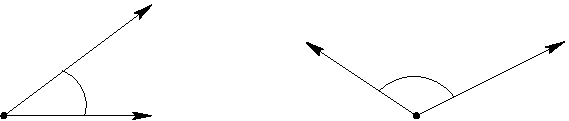
\includegraphics[scale=.8]{figures/vectors-14.pdf}}
\put(1.1,0.45){\small $\vec{u}$}
\put(1.1,0.0){\small $\vec{v}$}
\put(1.3,0.25){\small $\theta$}
\put(2.6,0.2){\small $\vec{u}$}
\put(3.4,0.2){\small $\vec{v}$}
\put(3.0,0.4){\small $\theta$}
\end{picture}

\uncover<2->{
\begin{theorem}\em
Let $\vec{u}$ and $\vec{v}$ be nonzero vectors, and let 
$\theta$ denote the angle between $\vec{u}$ and $\vec{v}$.
Then
\[ \vec{u}\dotprod\vec{v} =  \vectlength \vec{u} \vectlength ~ \vectlength \vec{v} \vectlength \cos\theta.\]
\end{theorem}}


}
%-------------- end slide -------------------------------%

%----------------start slide--------------------%
\frame{
\begin{alertblock}{Finding the included angle for nonzero vectors}
As a consequence of the Theorem, if $\vec{u}$ and $\vec{v}$ are
nonzero vectors with included angle $\theta$, 
then $\|\vec{u}\|\neq 0$ and $\|\vec{v}\|\neq 0$,
 
and 
\[ \cos\theta =\frac{\vec{u}\bullet\vec{v}}{\|\vec{u}\|\|\vec{v}\|}.\]
\pause
\begin{enumerate}
\item If $0\leq\theta <\frac{\pi}{2}$, then $\cos\theta >0$, 
\pause
implying that $\vec{u}\bullet\vec{v}> 0$.
\pause
Conversely, if $\vec{u}\bullet\vec{v}> 0$, then
$0\leq\theta <\frac{\pi}{2}$.
\pause
\item If $\theta=\frac{\pi}{2}$, then $\cos\theta =0$,
\pause
implying that $\vec{u}\bullet\vec{v}=0$.
\pause
Conversely, if $\vec{u}\bullet\vec{v}= 0$, then
$\theta =\frac{\pi}{2}$.
\pause
\item If $\frac{\pi}{2}<\theta\leq\pi$, then $\cos\theta <0$,
\pause
implying that $\vec{u}\bullet\vec{v}<0$.
\pause
Conversely, if $\vec{u}\bullet\vec{v}< 0$, then
$\frac{\pi}{2}<\theta\leq\pi$.
\end{enumerate}
\end{alertblock}
}
%----------------------end slide-------------------%


%-------------- start slide -------------------------------%
\frame{\frametitle{Included Angle}
\begin{problem}\em
Find the angle between
$\vec{u}=
\left[\begin{array}{r}
1 \\ 0 \\ -1 
\end{array}\right]$ 
and
$\vec{v}=
\left[\begin{array}{r}
0 \\ 1 \\ -1 
\end{array}\right]$.
\end{problem}
\medskip

\uncover<2->{
\begin{solution}\em

$\vec{u}\dotprod\vec{v}=1$,
$\vectlength \vec{u} \vectlength =\sqrt{2}$ and $\vectlength \vec{v} \vectlength =\sqrt{2}$.

Therefore, 
\[ \cos\theta = \frac{\vec{u}\dotprod\vec{v}}
{\vectlength \vec{u} \vectlength ~ \vectlength \vec{v} \vectlength}
= \frac{1}{\sqrt{2}\sqrt{2}}=\frac{1}{2}.  \]

Since $0\leq\theta\leq\pi$, 
$\theta = \frac{\pi}{3}$.
\bigskip

Therefore, the angle between $\vec{u}$ and $\vec{v}$ is
$\frac{\pi}{3}$.
\end{solution}}
}
%-------------- end slide -------------------------------%

%--------------------start slide-------------------------%
\frame{
\begin{problem}\em
Find the included angle for 
$\vect{u} = \left[ \begin{array}{r}
3 \\ -6 \\ -3 \end{array}\right]$
and
$\vect{v} = \left[ \begin{array}{r}
-2 \\ 1 \\ -1 \end{array}\right]$. 
\end{problem}
\pause
\begin{solution}\em
\[ \vec{u} \bullet \vec{v} = \pause -9,~
\pause
\|\vec{u}\| \pause =\sqrt{54}\pause = 3\sqrt{6},
\pause
~\mbox{ and }~
\|\vec{v}\| \pause =\sqrt{6}.
\]
\pause
Let $\theta$ denote the included angle for $\vec{u}$
and $\vec{v}$.
\pause
Then
\[ \cos\theta=\frac{\vec{u} \bullet \vec{v}}
{\|\vec{u}\|\|\vec{v}\|} 
\pause
=\frac{-9}{3\sqrt{6}\times\sqrt{6}}
\pause
=\frac{-9}{18}
\pause
=-\frac{1}{2}.  \]
\pause
Since $0\leq \theta\leq \pi$, the included angle is 
$\theta=\frac{2\pi}{3}$.
\end{solution}
}
%----------------------end slide------------------------%

%--------------------start slide-------------------------%
\frame{
\begin{problem}\em
Find the included angle for
$\vec{u}=
\left[\begin{array}{r}
7 \\ -1 \\ 3
\end{array}\right]$
and
$\vec{v}=
\left[\begin{array}{r}
1 \\ 4 \\ -1
\end{array}\right]$.
\end{problem}
\pause
\begin{solution}\em
Let $\theta$ denote included angle.
\pause
\[ \vec{u}\bullet\vec{v}=\pause 0.\]
\pause
Regardless of $\|\vec{u}\|$ and $\|\vec{v}\|$, 
$\cos\theta = 0$,
\pause
and therefore the included angle is $\theta=\frac{\pi}{2}$.
\end{solution}
}
%----------------------end slide------------------------%


%-------------- start slide -------------------------------%
\frame{\frametitle{Orthogonal Vectors}
\begin{definition}
Vectors $\vec{u}$ and $\vec{v}$ are \alert{orthogonal}, also called perpendicular,
if and only if $\vec{u}=\vec{0}$ or $\vec{v}=\vec{0}$
or $\theta=\frac{\pi}{2}$.
\end{definition}
\bigskip

\pause
\begin{theorem}\em
Nonzero vectors $\vec{u}$ and $\vec{v}$ are orthogonal if
and only if $\vec{u}\dotprod\vec{v}=0$.
\end{theorem}

\pause
\begin{block}{Proof} 
We have $\vec{u}\perp \vec{v}$ if and only if $\|\vec{u}-\vec{v}\|=\|\vec{u}+\vec{v}\|$ (see the picture). 

This is equivalent to 
\[
(\vec{u}-\vec{v})\bullet
(\vec{u}-\vec{v})=
(\vec{u}+\vec{v})\bullet
(\vec{u}+\vec{v})
\]
which gives $-2\vec{u}\bullet\vec{v}=2\vec{u}\bullet\vec{v}$ and therefore $\vec{u}\bullet \vec{v}=0$. 
\end{block} 
}
%-------------- end slide -------------------------------%


%-------------- start slide -------------------------------%
\frame{
\begin{problem}\em
Find all vectors $\vec{v}=
\left[\begin{array}{r}
x \\ y \\ z
\end{array}\right]$
orthogonal to both
$
\vec{u}=
\left[\begin{array}{r}
-1 \\ -3 \\ 2
\end{array}\right]$ and $
\vec{w}=
\left[\begin{array}{r}
0 \\ 1 \\ 1
\end{array}\right]$
\end{problem}

\uncover<2->{
\begin{solution}\em
There are infinitely many such vectors.}

\uncover<3->{
Since $\vec{v}$ is orthogonal to both $\vec{u}$ and $\vec{w}$,
\[ \begin{array}{rcl}
\vec{v}\dotprod\vec{u} & = & -x-3y+2z=0 \\
\vec{v}\dotprod\vec{w} & = & y+z=0 
\end{array}\]

\end{solution}}
}
%-------------- end slide -------------------------------%

%-------------- start slide -------------------------------%
\frame{
\begin{solution}[continued]\em
This is a homogeneous system of two linear equation in three
variables.
\[
\left[\begin{array}{rrr|r}
-1 & -3 & 2 & 0 \\
0 & 1 & 1 & 0 
\end{array}\right]
\rightarrow \cdots \rightarrow
\left[\begin{array}{rrr|r}
1 & 0 & -5 & 0 \\
0 & 1 & 1 & 0 
\end{array}\right]
\]

\pause

$\left[\begin{array}{rrr|r}
1 & 0 & -5 & 0 \\
0 & 1 & 1 & 0
\end{array}\right]$
implies that
$\vec{v}=\left[\begin{array}{r}
5t \\ -t \\ t
\end{array}\right]$ for $t\in\RR$.

\pause

Therefore,
$\vec{v}=t\left[\begin{array}{r}
5 \\ -1 \\ 1
\end{array}\right]$ for all $t\in\RR$.
\end{solution}
}
%-------------- end slide -------------------------------%

%-------------- start slide -------------------------------%
\frame{
\begin{problem}\em
Are $A(4,-7,9)$, $B(6,4,4)$ and $C(7,10,-6)$ the vertices of
a right angle triangle?
\end{problem}
\uncover<2->{
\begin{solution}\em

\[
\overrightarrow{AB} =
\left[\begin{array}{r}
2 \\ 11 \\ -5
\end{array}\right],
\overrightarrow{AC} =
\left[\begin{array}{r}
3 \\ 17 \\ -15
\end{array}\right],
\overrightarrow{BC} =
\left[\begin{array}{r}
1 \\ 6 \\ -10
\end{array}\right] \]}

\begin{itemize}
\item<3->
$\overrightarrow{AB}\dotprod \overrightarrow{AC}
= 6 + 187 + 75 \neq 0$.
\item<4->
$\overrightarrow{BA}\dotprod \overrightarrow{BC}
= (-\overrightarrow{AB})\dotprod \overrightarrow{BC}
= -2 -66-50 \neq 0$.
\item<5->
$\overrightarrow{CA}\dotprod \overrightarrow{CB} 
= (-\overrightarrow{AC})\dotprod (-\overrightarrow{BC}) 
= \overrightarrow{AC}\dotprod \overrightarrow{BC} 
=3+102+150\neq 0$.
\end{itemize}

\uncover<6->{
None of the angles is $\frac{\pi}{2}$, and therefore
the triangle is not a right angle triangle.}
\end{solution}

}
%-------------- end slide -------------------------------%

%-------------- start slide -------------------------------%
\frame{
\begin{problem}\em
A rhombus is a parallelogram with sides of equal length.  
Prove that the diagonals of a rhombus are perpendicular.
\end{problem}
\uncover<2->{
\begin{solution}\em

\begin{picture}(4,.9)
\put(0.4,0.1){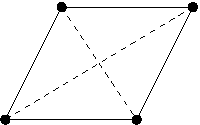
\includegraphics[scale=.8]{figures/vectors-15.pdf}}
\put(0.5,0.5){\small $\vec{u}$}
\put(0.8,0.0){\small $\vec{v}$}
\put(1.7,0.8){\small Define the parallelogram (rhombus) by }
\put(1.7,0.6){\small vectors $\vec{u}$ and $\vec{v}$.}
\put(1.7,0.3){\small Then the diagonals are $\vec{u}+\vec{v}$
and $\vec{u}-\vec{v}$.}
\put(1.7,0.0){\small Show that $\vec{u}+\vec{v}$ and
$\vec{u}-\vec{v}$ are perpendicular.}
\end{picture}

\uncover<3->{
\begin{eqnarray*}
(\vec{u}+\vec{v})\dotprod(\vec{u}-\vec{v})
& = & \vec{u}\dotprod\vec{u}-\vec{u}\dotprod\vec{v} 
+ \vec{v}\dotprod\vec{u} - \vec{v}\dotprod\vec{v} \\
& = & \vectlength \vec{u} \vectlength ^2 -\vec{u}\dotprod\vec{v} + \vec{u}\dotprod\vec{v}
- \vectlength \vec{v} \vectlength ^2 \\
& = & \vectlength \vec{u} \vectlength ^2 - \vectlength \vec{v} \vectlength ^2 \\
& = & 0, \mbox{ since } \vectlength \vec{u} \vectlength = \vectlength \vec{v}\vectlength.
\end{eqnarray*}

Therefore, the diagonals are perpendicular.}
}
\end{solution}
}
%-------------- end slide -------------------------------%

\section{Projections}

%-------------- start slide -------------------------------%
\frame{\frametitle{Projections}

\begin{theorem}\em
Given nonzero vectors $\vec{v}$ and $\vec{u}$ in $\mathbb{R}^n$(for $n=2,3...$), there exist unique vectors $\vect{v}_{||}, \vect{v}_{\perp}$ such that $\vec{v}$ can be written  
as a sum
\[
\vec{v}=\vec{v}_{||}+ \vec{v}_{\perp}
\]

where \textcolor{blue}{$\vec{v}_{||}$ is parallel to $\vec{u}$} and 
\alert{$\vec{v}_{\perp}$ is orthogonal to $\vec{u}$.}
\end{theorem}

\uncover<2->{
\begin{picture}(3,.9)
\put(0.3,0.1){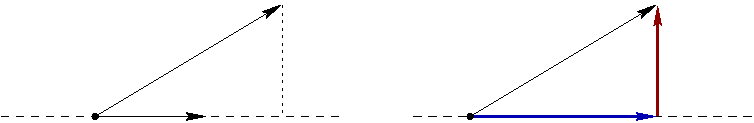
\includegraphics[scale=.8]{figures/vectors-16.pdf}}
\put(1.05,-0.05){\small $\vec{u}$}
\put(1.25,0.5){\small $\vec{v}$}
\put(3.25,0.0){\small $\vec{v}_{||}$}
\put(3.25,0.5){\small $\vec{v}$}
\put(3.85,0.3){\small $\vec{v}_{\perp}$}
\end{picture}
}
\medskip

\uncover<3->{
$\vec{v}_{||}$ is \alert{the projection of $\vec{v}$ onto 
$\vec{u}$}, written
$\vec{v}_{||} = \proj_{\vec{u}} \vec{v}$ and $\vec{v}_{\perp} = \vec{v} - \vec{v}_{||}$. }


}
%-------------- end slide -------------------------------%


%-------------- start slide -------------------------------%
\frame{\frametitle{Projections}
\begin{block}{A formula for $\proj_{\vec{u}} \vec{v}$}
The defining properties of $\vec{v}_{||}$ and $\vec{v}_{\perp}$ are
\pause
\begin{enumerate}
\item $\vec{v}_{||}$ is parallel to $\vec{u}$;
\pause
\item $\vec{v}_{\perp}$ is orthogonal to $\vec{u}$;
\pause
\item $\vec{v}_{||}+\vec{v}_{\perp}=\vec{v}$.
\end{enumerate}
\pause
Since $\vec{v}_{||}$ is parallel to $\vec{u}$,
$\vec{v}_{||}=t\vec{u}$ for some $t\in\RR$.
\pause
Furthermore,
$\vec{v}_{\perp} = \vec{v}-\vec{v}_{||}$ and $\vec{v}_{\perp}$ is orthogonal to $\vec{u}$,
\pause
so
\[ 0 = \vec{v}_{\perp}\dotprod\vec{u}
\pause
=(\vec{v}-\vec{v}_{||})\dotprod \vec{u}
\pause
=(\vec{v}-t\vec{u})\dotprod \vec{u}
\pause
=\vec{v}\dotprod\vec{u} - t(\vec{u}\dotprod\vec{u}).\]
\pause
Since $\vec{u}\neq \vec{0}$, it follows that
$t=\frac{\vec{v}\dotprod\vec{u}}{\vectlength \vec{u} \vectlength ^{2}}$.
\pause
Therefore
\[ \vec{v}_{||}=\left( \frac{\vec{v}\dotprod\vec{u}}
{\vectlength \vec{u}\vectlength^2} \right) \vec{u},
\pause
~\mbox{ and }~
\vec{v}_{\perp}=\vec{v}- \left( \frac{\vec{v}\dotprod\vec{u}}
{\vectlength \vec{u}\vectlength ^2} \right) \vec{u}.\]
\end{block}
}
%------------------------end slide------------------------%

%-------------------start slide-------------------------%
\frame{\frametitle{Projections}

\begin{theorem}\em
Let $\vec{v}$ and $\vec{u}$ be vectors with $\vec{u}\neq\vec{0}$.
\begin{enumerate}
\item
$ \proj_{\vec{u}}\vec{v}
= \left(  \frac{\vec{v}\dotprod\vec{u}}{\vectlength \vec{u} \vectlength^2} \right) \vec{u}$
\item
$ \vec{v}- \left( \frac{\vec{v}\dotprod\vec{u}}{\vectlength \vec{u} \vectlength^2}  \right) \vec{u}$
is orthogonal to $\vec{u}$.
\end{enumerate}
\end{theorem}
}

%-------------- end slide -------------------------------%

%-------------- start slide -------------------------------%
\frame{
\begin{problem}\em
Let $\vec{v}=\left[\begin{array}{r}
2 \\ -1 \\ 0 \end{array}\right]$
and
$\vec{u}=\left[\begin{array}{r}
3 \\ 1 \\ -1 \end{array}\right]$.
Find vectors $\vec{v}_{||}$ and $\vec{v}_{\perp}$ so that 
$\vec{v}=\vec{v}_{||} + \vec{v}_{\perp}$, with
$\vec{v}_{||}$ parallel to $\vec{u}$ and
$\vec{v}_{\perp}$ orthogonal to $\vec{u}$.
\end{problem}
\medskip

\uncover<2->{
\begin{solution}\em
\[
\vec{v}_{||}=\proj_{\vec{u}} \vec{v} =
\left( \frac{\vec{v}\dotprod\vec{u}}{\vectlength \vec{u} \vectlength^2} \right) \vec{u}
= \frac{5}{11} 
\left[\begin{array}{r}
3 \\ 1 \\ -1 \end{array}\right]
=\left[\begin{array}{r}
15/11 \\ 5/11 \\ -5/11 \end{array}\right].\] }

\uncover<3->{
\[
\vec{v}_{\perp}=\vec{v}-\vec{v}_{||}
=\left[\begin{array}{r}
2 \\ -1 \\ 0 \end{array}\right]
-
\frac{5}{11} 
\left[\begin{array}{r}
3 \\ 1 \\ -1 \end{array}\right]
=
\frac{1}{11} 
\left[\begin{array}{r}
7 \\ -16 \\ 5 \end{array}\right]
=\left[\begin{array}{r}
7/11 \\ -16/11 \\ 5/11 \end{array}\right].
\]}

\end{solution}
}

%-------------- start slide -------------------------------%
\frame{\frametitle{Distance from a Point to a Line}
\begin{problem}\em
Let $P=(3,2,-1)$ be a point in $\RR^3$ and $L$ a line with
equation
\[ 
\left[\begin{array}{c}
x \\ y \\ z \end{array}\right]
=
\left[\begin{array}{r}
2 \\ 1 \\ 3 \end{array}\right]
+
t\left[\begin{array}{r}
3 \\ -1 \\ -2 \end{array}\right].\]
Find the shortest distance from $P$ to $L$, and find the point
$Q$ on $L$ that is closest to $P$.
\end{problem}

\uncover<2->{
\begin{solution}\em

\begin{picture}(4,1.2)
\put(0.2,0.2){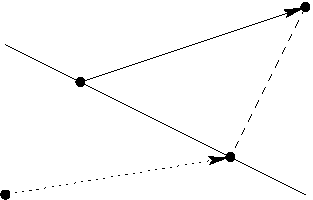
\includegraphics[scale=.7]{figures/vectors-17.pdf}}
\put(0.1,0.2){\small $0$}
\put(0.2,0.7){\small $L$}
\put(0.5,0.6){\small $P_0$}
\put(1.65,1.05){\small $P$}
\put(1.2,0.25){\small $Q$}
\put(1.0,0.95){\small $\vec{u}$}
\put(2.1,1.2){\small Let $P_0=(2,1,3)$ be a point on $L$,}
\put(2.1,1.0){\small and let
$\vec{d}= \left[\begin{array}{ccc}
3 & -1 & -2 \end{array}\right]^T$.}
\put(2.1,0.8){\small Then $\overrightarrow{P_0Q}
=\proj_{\vec{d}}\overrightarrow{P_0P}$,
$\overrightarrow{0Q}=\overrightarrow{0P_0} +
\overrightarrow{P_0Q}$,}
\put(2.1,0.6){\small and the shortest distance from $P$ to $L$ is}
\put(2.1,0.4){\small the length of $\overrightarrow{QP}$, where
$\overrightarrow{QP} = 
\overrightarrow{P_0P}-\overrightarrow{P_0Q}$.}
\end{picture}
}
\end{solution}
}
%-------------- end slide -------------------------------%

%-------------- start slide -------------------------------%
\frame{
\begin{solution}[continued]\em
$\overrightarrow{P_0P}= \left[\begin{array}{r}
1 \\
1 \\
-4 \end{array}\right]$,
$\vec{d}= \left[\begin{array}{r}
3 \\
-1 \\
-2 
\end{array}\right]$.
\[
\overrightarrow{P_0Q}= \proj_{\vec{d}}\overrightarrow{P_0P} 
= \left( \frac{\overrightarrow{P_0P}\dotprod\vec{d}}{\vectlength \vec{d} \vectlength^2} \right) \vec{d} 
= \frac{10}{14}
\left[\begin{array}{r}
3 \\ -1 \\ -2 \end{array}\right]
=\frac{1}{7}
\left[\begin{array}{r}
15 \\ -5 \\ -10 \end{array}\right].
\]

\uncover<2->{
Therefore,
\[ \overrightarrow{0Q}=
\left[\begin{array}{c}
2 \\ 1 \\ 3 \end{array}\right]
+ \frac{1}{7}
\left[\begin{array}{r}
15 \\ -5 \\ -10 \end{array}\right]
=
\frac{1}{7}
\left[\begin{array}{r}
29 \\ 2 \\ 11 \end{array}\right],
\]
so $Q=\left(\frac{29}{7}, \frac{2}{7}, \frac{11}{7}\right)$.
}
\end{solution}
}

%-------------- end slide -------------------------------%

%-------------- start slide -------------------------------%
\frame{
\begin{solution}[continued]\em
Finally, the shortest distance from $P(3,2,-1)$ to $L$ is the 
length of $\overrightarrow{QP}$, where
\[ \overrightarrow{QP} =                     
\overrightarrow{P_0P}-\overrightarrow{P_0Q}
=
\left[\begin{array}{r}
1 \\ 1 \\ -4 \end{array}\right] 
-
\frac{1}{7}
\left[\begin{array}{r}
15 \\ -5 \\ -10 \end{array}\right]
=
\frac{2}{7}
\left[\begin{array}{r}
-4 \\ 6 \\ -9 \end{array}\right].
\]

\uncover<2->{
Therefore the shortest distance from $P$ to $L$ is
\[ \vectlength \overrightarrow{QP} \vectlength =
\frac{2}{7}\sqrt{(-4)^2 + 6^2 + (-9)^2}
=\frac{2}{7}\sqrt{133}.\]}
\end{solution}

}
%-------------- end slide -------------------------------%

\end{document}
